\section{Data collection methodology}
\label{section:experiments}

To collect the data, we have used two identical WiFi adapters 
(supporting IEEE 802.11ac standard), two microcomputers, and a 
GPS receiver. We have configured the adapters with maximum output 
power (20dBm) and used 3dBi omnidirectional antennas. 

We have logged the GPS coordinates and WiFi signal strengths every 1 
second and stored the collected data in the file. We have chosen large enough open-space
outside of the city to collect the data so that the interference at 5GHz range was minimized.


\begin{figure}[h!]
\centering
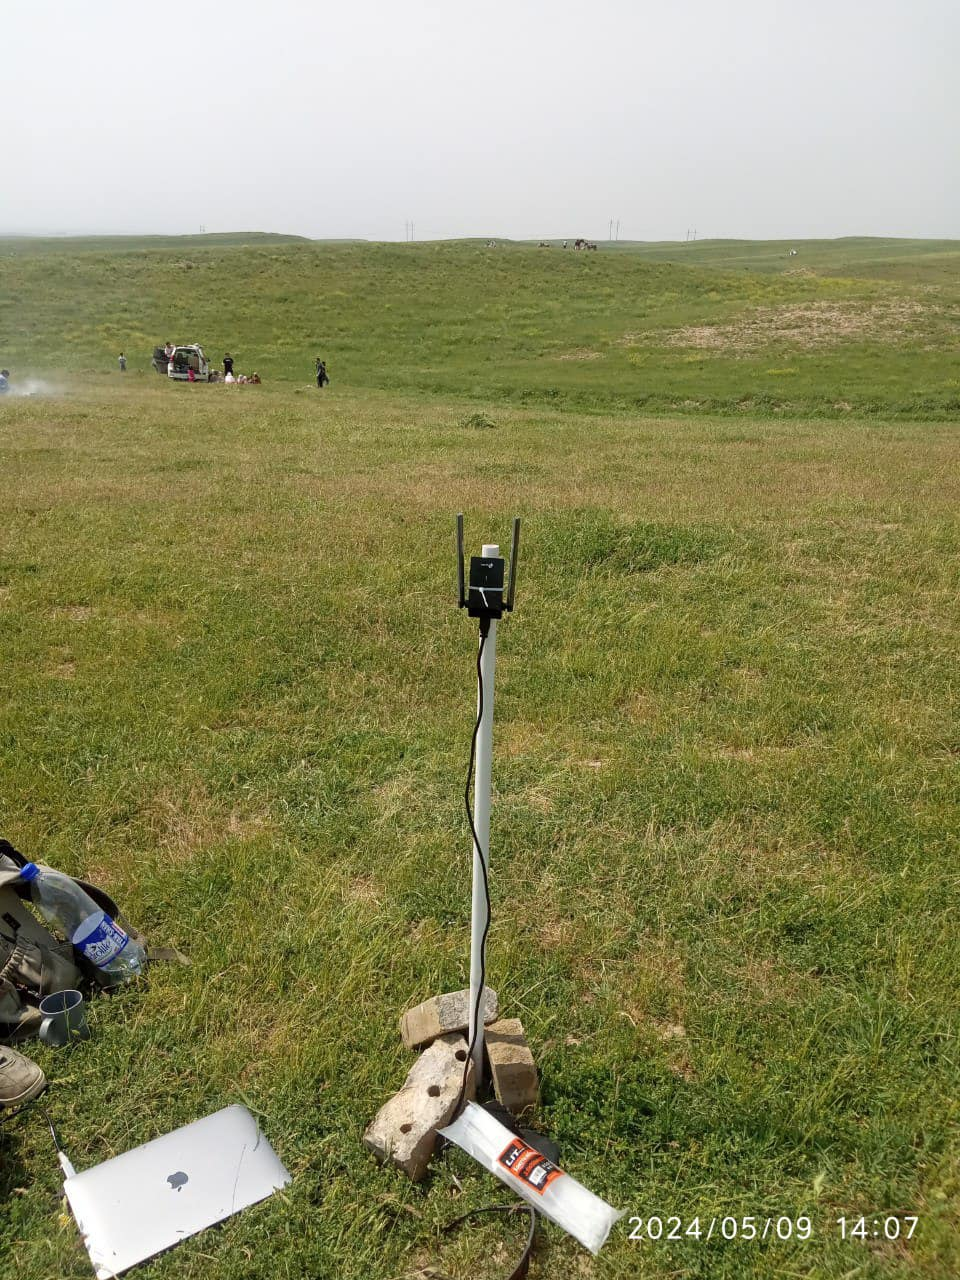
\includegraphics[width=0.4\textwidth]{graphics/wifi_outdoor.jpg}
\caption{WiFi base station}
\label{fig:basestion}
\end{figure}

